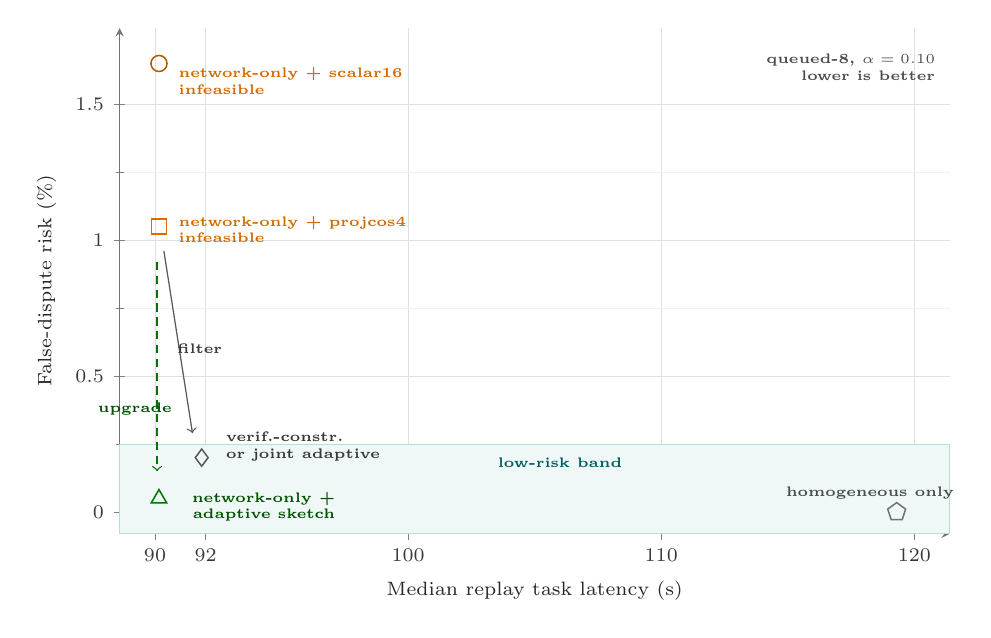
\begin{tikzpicture}
\begin{axis}[
	width=\linewidth,
	height=0.66\linewidth,
	xmin=88.6,
	xmax=121.4,
	ymin=-0.08,
	ymax=1.78,
	axis lines=left,
	axis line style={black!55,line width=0.35pt},
	grid=both,
	major grid style={black!12,line width=0.25pt},
	minor grid style={black!6,line width=0.18pt},
	minor x tick num=1,
	minor y tick num=1,
	xlabel={Median replay task latency (s)},
	ylabel={False-dispute risk (\%)},
	xlabel style={font=\scriptsize,text=black!85},
	ylabel style={font=\scriptsize,text=black!85},
	tick label style={font=\scriptsize,text=black!78},
	xtick={90,92,100,110,120},
	ytick={0,0.5,1.0,1.5},
	enlarge x limits=false,
	clip=false,
]
\path[fill=teal!6,draw=teal!28,line width=0.25pt]
	(axis cs:88.6,-0.08) rectangle (axis cs:121.4,0.25);
\node[anchor=center,font=\tiny\bfseries,text=teal!72!black] at (axis cs:106.0,0.18)
	{low-risk band};

\addplot+[only marks,mark=o,mark size=2.9pt,
	draw=orange!70!black,
	mark options={solid,draw=orange!70!black,fill=white,line width=0.55pt}]
	coordinates {(90.156,1.65)};
\node[anchor=south west,font=\tiny\bfseries,align=left,text=orange!82!black]
	at (axis cs:90.55,1.50) {network-only + scalar16\\infeasible};

\addplot+[only marks,mark=square,mark size=2.7pt,
	draw=orange!85!black,
	mark options={solid,draw=orange!85!black,fill=white,line width=0.55pt}]
	coordinates {(90.156,1.05)};
\node[anchor=west,font=\tiny\bfseries,align=left,text=orange!82!black]
	at (axis cs:90.55,1.04) {network-only + projcos4\\infeasible};

\addplot+[only marks,mark=triangle,mark size=3.2pt,
	draw=green!45!black,
	mark options={solid,draw=green!45!black,fill=white,line width=0.55pt}]
	coordinates {(90.156,0.05)};
\node[anchor=east,font=\tiny\bfseries,align=right,text=green!32!black]
	at (axis cs:97.5,0.02) {network-only + \\ adaptive sketch};

\addplot+[only marks,mark=diamond,mark size=3.1pt,
	draw=black!65,
	mark options={solid,draw=black!65,fill=white,line width=0.55pt}]
	coordinates {(91.844,0.20)};
\node[anchor=west,font=\tiny\bfseries,align=left,text=black!78]
	at (axis cs:92.42,0.24) {verif.-constr.\\or joint adaptive};

\addplot+[only marks,mark=pentagon,mark size=3.4pt,line width=0.7pt,
	draw=black!55,
	mark options={solid,draw=black!55,fill=white,line width=0.55pt}]
	coordinates {(119.301,0.00)};
\node[anchor=south east,font=\tiny\bfseries,align=right,text=black!70]
	at (axis cs:121.95,0.01) {homogeneous only};

\draw[->,line width=0.45pt,black!65]
	(axis cs:90.35,0.96) -- (axis cs:91.48,0.29);
\node[anchor=west,font=\tiny\bfseries,text=black!78]
	at (axis cs:90.5,0.60) {filter};

\draw[->,line width=0.45pt,densely dashed,green!45!black]
	(axis cs:90.08,0.92) -- (axis cs:90.08,0.15);
\node[anchor=west,font=\tiny\bfseries,text=green!32!black]
	at (axis cs:87.36,0.38) {upgrade};

\node[anchor=north east,font=\tiny\bfseries,align=right,text=black!70]
	at (axis cs:121.2,1.72) {queued-8, $\alpha=0.10$\\lower is better};
\end{axis}
\end{tikzpicture}
